%=============================================================================
%  A Causally-Grounded Decision System for Retail Profit Optimisation
%  IEEE conference format (IEEEtran, conference option)
%
%  BUILD
%    pdflatex main
%    pdflatex main            (twice, so cross-references resolve)
%
%  The main paper is EXACTLY 6 pages. The appendix listing that follows the
%  references is intentionally outside that limit.
%=============================================================================
\documentclass[conference]{IEEEtran}
\IEEEoverridecommandlockouts

% T1 encoding is REQUIRED here. The default OT1 encoding has no glyph for the
% straight double quote, so every " in the appendix code raised
% "\textquotedbl unavailable in encoding OT1".
\usepackage[T1]{fontenc}
\usepackage[utf8]{inputenc}

\usepackage{cite}
\usepackage{amsmath,amssymb}
\usepackage{graphicx}
\usepackage{booktabs}
\usepackage{url}
\usepackage{balance}

% fvextra gives us VerbatimInput with line breaking. We deliberately do NOT
% use the listings package: listings runs a syntax lexer over every line, and
% across 3,552 lines of Python that exceeded the Overleaf free-tier compile
% budget. Verbatim typesetting is an order of magnitude cheaper and is immune
% to whatever characters happen to appear in the source.
\usepackage{fvextra}

\graphicspath{{figures/}}

% ---------------------------------------------------------------------------
% Float placement tuning. LaTeX's defaults are conservative: a page carrying a
% double-column float may use at most 70% of its height for it, and must keep
% 20% for text. With five wide floats that rule left large gaps and deferred
% figures, costing roughly a page of whitespace. These values let a float fill
% more of the page and shrink the space around it.
% ---------------------------------------------------------------------------
\renewcommand{\topfraction}{0.95}
\renewcommand{\bottomfraction}{0.95}
\renewcommand{\textfraction}{0.05}
\renewcommand{\floatpagefraction}{0.88}
\renewcommand{\dbltopfraction}{0.95}
\renewcommand{\dblfloatpagefraction}{0.88}
\setlength{\textfloatsep}{7pt plus 2pt minus 2pt}
\setlength{\floatsep}{7pt plus 2pt minus 2pt}
\setlength{\dblfloatsep}{7pt plus 2pt minus 2pt}
\setlength{\dbltextfloatsep}{7pt plus 2pt minus 2pt}
\setcounter{topnumber}{3}
\setcounter{dbltopnumber}{3}
\setcounter{totalnumber}{4}

% ---------------------------------------------------------------------------
% Appendix switch.
%   \includecodetrue   -> 6-page paper + full code appendix   (default)
%   \includecodefalse  -> 6-page paper only, compiles in seconds
% Flip this if the appendix ever times out again.
% ---------------------------------------------------------------------------
\newif\ifincludecode
\includecodetrue

\newcommand{\codefile}[2]{%
  \vspace{3mm}\noindent\textbf{\texttt{#1}}\par\vspace{1mm}%
  \VerbatimInput[fontsize=\tiny, numbers=left, numbersep=4pt,
                 breaklines=true, breakanywhere=true, obeytabs=true,
                 frame=leftline, framesep=2mm, xleftmargin=7mm]{code/#2}}

\begin{document}

%=============================================================================
\title{A Causally-Grounded Decision System for Retail\\Profit Optimisation:
Elasticity, Promotion Uplift,\\Markdown and Replenishment}

% ---------------------------------------------------------------------------
% AUTHOR BLOCK
% Confirm the campus city on line three if you are not at the Vellore campus.
% ---------------------------------------------------------------------------
\author{\IEEEauthorblockN{Varshni K}
\IEEEauthorblockA{\textit{School of Computer Science and Engineering} \\
\textit{Vellore Institute of Technology} \\
Vellore, India \\
varshni.k2024@vitstudent.ac.in}}

\maketitle

%=============================================================================
\begin{abstract}
Retail analytics projects usually stop at prediction, reporting forecast
accuracy but never showing that acting on the model would have earned money.
This paper describes an end-to-end decision system built on 524{,}926
store--week--product records from the dunnhumby \emph{Breakfast at the Frat}
panel, covering 55 products across 77 stores over 156 weeks. Five estimation
and decision modules are chained together: own-price elasticity estimated with
a Hausman instrument and empirical-Bayes shrinkage; promotion uplift measured
by two-way fixed-effects difference-in-differences; a gradient-boosted demand
forecast with a smearing correction; constrained price optimisation; markdown
scheduling by backward induction; and forecast-driven replenishment. Every
estimator is validated twice, once against the real panel and once against a
schema-identical synthetic replica in which the true elasticity and true
promotional lift are known by construction. On that replica the naive
promotion estimate is biased by $0.557$ in log-lift while the
difference-in-differences estimate is biased by $0.010$. On the real data the
share of products with economically impossible positive elasticity falls from
$5.5\%$ to $0\%$, the forecast improves on the strongest naive baseline by
$30.5\%$ in WAPE, markdown scheduling recovers $6.6\%$ more cash than a fixed
discount ladder, and forecast-driven replenishment cuts inventory cost by
$48.1\%$ while raising fill rate.
\end{abstract}

\begin{IEEEkeywords}
retail analytics, price elasticity, instrumental variables,
difference-in-differences, demand forecasting, markdown optimisation,
inventory replenishment
\end{IEEEkeywords}

%=============================================================================
\section{Introduction}

A supermarket chain decides weekly, for every product in every store, what
price to charge, whether to promote, how deep to discount ageing stock and how
much to reorder. Each decision moves gross profit and depends on the others: a
promotion changes demand, that changes the reorder quantity, and the discount
driving the promotion consumes the margin the reorder was meant to earn.

Most work on this problem is organised around prediction: a demand model is
fitted, an accuracy figure is reported, and the project ends. Two things are
missing. First, prediction and decision are not the same task --- knowing that
units rise when price falls says nothing about whether price should fall.
Second, the quantities such systems rely on are biased in a known direction,
because prices and promotions are not set at random.

Retailers cut prices in weeks when they already expect strong demand, and
promote harder in stores that are already busy, so price is correlated with the
demand shock and least squares confounds the two. In the panel used here a
plain log--log regression returns a \emph{positive} own-price elasticity for
$5.5\%$ of products, implying that raising price sells more; a naive
before-and-after comparison overstates an in-store display by over a factor of
two.

This paper describes a system built to avoid that failure mode. The
contributions are:

\begin{itemize}
\item an elasticity estimator combining store fixed effects, a Hausman
      instrument formed from the same product's price in other stores, and
      empirical-Bayes shrinkage, which removes all economically impossible
      estimates from the panel;
\item a promotion-uplift model that separates the effect of the merchandising
      mechanic from the effect of the accompanying price cut, with an explicit
      parallel-trends placebo test;
\item three decision modules --- constrained pricing, markdown scheduling by
      backward induction, and forecast-driven replenishment --- each benchmarked
      against the incumbent heuristic, and for inventory against a
      perfect-foresight bound;
\item a validation design running every estimator on a schema-identical
      synthetic replica with known parameters, so estimator quality is measured
      rather than asserted.
\end{itemize}

The last point makes the rest credible. On real data the true elasticity is
unobservable, so internal consistency proves nothing; running identical code on
data whose parameters were fixed in advance turns that into a measurement.

%=============================================================================
\section{Related Work}

\subsection{Demand forecasting in retail}
Gradient-boosted trees remain a strong default for the tabular, count-valued
series retail produces \cite{friedman2001}. Recent work couples forecasting
directly to inventory decisions rather than treating them separately
\cite{yang2025}, the arrangement adopted here.

\subsection{Price elasticity and endogeneity}
That observed prices are endogenous to demand is long established. Nevo's
analysis of ready-to-eat cereal \cite{nevo2001} is directly relevant, both
methodologically and because cereal is one of our four categories. The standard
remedy is an instrument correlated with cost but not local demand, canonically
the same product's price in other markets; strength is judged by the first-stage
$F$ against a threshold of ten \cite{stock2005}. Where per-product estimates are
noisy, empirical-Bayes shrinkage reduces total error \cite{efron1973}.

\subsection{Promotion effect measurement}
Separating what a promotion caused from what merely coincided with it is a
causal-inference problem. Difference-in-differences with two-way fixed effects
is the standard panel approach \cite{angrist2009}, resting on a parallel-trends
assumption that should be tested rather than assumed \cite{bertrand2004}. Causal
methods are increasingly used for marketing targeting \cite{lemmens2025}.

\subsection{Pricing, markdown and inventory decisions}
The profit-maximising price under constant-elasticity demand follows the Lerner
condition \cite{lerner1934}. Clearance with fixed stock and a deadline is a
different problem, solved classically by dynamic programming
\cite{gallego1994}. For replenishment, deep reinforcement learning
has been found competitive rather than dominant against established heuristics
\cite{gijsbrechts2022}, motivating our use of exact dynamic programming where
the transition model is known. Unconstrained algorithmic pricing empirically
raises margins in ways consistent with weakened competition \cite{assad2024},
and autonomous agents can reach supra-competitive prices without explicit
coordination \cite{fish2024}; both argue for hard guardrails. Explainability
requirements are surveyed in \cite{debock2024}.

\subsection{Summary and research gap}
Each component is individually well studied. What is uncommon is a single
pipeline in which causal estimates feed decision modules, decisions are scored
on held-out weeks against the incumbent heuristic, and the estimators are
themselves validated against known ground truth. That combination is the gap
addressed here.

%=============================================================================
\begin{figure*}[!t]
\centering
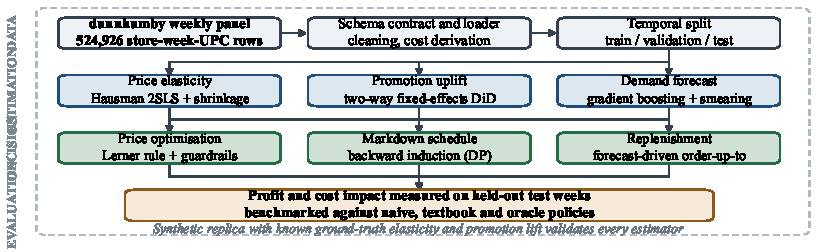
\includegraphics[width=\textwidth]{fig1_architecture.pdf}
\caption{System architecture. Estimation feeds decision, which feeds
evaluation on held-out weeks. The dashed envelope is the synthetic replica on
which the identical pipeline is run against known ground truth.}
\label{fig:arch}
\end{figure*}

\section{Methodology}

\subsection{Problem formulation}
Let $q_{ist}$ be units of product $i$ sold in store $s$ in week $t$ at shelf
price $p_{ist}$ against reference price $b_{ist}$, with binary indicators
$F_{ist}$ (mailer), $D_{ist}$ (display) and $R_{ist}$ (temporary price
reduction), and unit cost $c_i$. The objective is gross profit $q(p-c)$, except
during clearance where it is cash recovered, the stock being already purchased.
Fig.~\ref{fig:arch} shows how the modules connect.

\subsection{Dataset and preprocessing}
The dunnhumby \emph{Breakfast at the Frat} panel \cite{dunnhumby} covers 156
weeks from January 2009 to December 2011 across cold cereal, frozen pizza, bag
snacks and oral hygiene. It is unusual among public retail datasets in reporting
shelf and reference price as separate fields, making discount depth directly
observable, and in carrying three merchandising flags rather than one.

Loading normalises the workbook to a fixed column contract and repairs
recoverable defects: 23 rows with null keys and one with non-positive units were
dropped, 6{,}232 rows whose reference price fell below shelf price were reset,
and two implying a discount deeper than $90\%$ were clipped
(Table~\ref{tab:data}).

Unit cost is absent, as no retailer publishes it; it is derived from a
per-category gross-margin assumption, and every dependent conclusion is
recomputed across a $\pm 5$ percentage-point band in
Section~\ref{sec:pricing}. Splits are strictly temporal --- weeks 1--110 train,
111--130 validation, 131--156 held out for a single final evaluation --- since a
random split would let later weeks inform earlier ones.

\begin{table}[!t]
\caption{Panel characteristics after cleaning}
\label{tab:data}
\centering
\footnotesize
\begin{tabular}{lr}
\toprule
Property & Value \\
\midrule
Store--week--product records & 524{,}926 \\
Stores & 77 \\
Products (UPC) & 55 \\
Weeks & 156 \\
Period & 2009-01-14 to 2012-01-04 \\
Records under any promotion & $28.5\%$ \\
Mean discount when promoted & $20.3\%$ \\
Median within-product price s.d. & $0.379$ \\
Train / validation / test rows & 368{,}410 / 70{,}010 / 86{,}506 \\
\bottomrule
\end{tabular}
\end{table}

\subsection{Elasticity estimation}
Demand is constant-elasticity, so in logs $\varepsilon_i$ is the coefficient on
log relative price. Three specifications are estimated per product. The first
regresses $\log q$ on $\log(p/b)$. The second adds store fixed effects, the
merchandising indicators, two seasonal harmonics and a linear trend. The third
addresses the remaining endogeneity, instrumenting own price by the
leave-one-out mean log price of the same product in \emph{other} stores in the
same week,
\begin{equation}
z_{ist}=\frac{1}{|S|-1}\sum_{s'\neq s}\log p_{is't}.
\label{eq:iv}
\end{equation}
The identifying argument is that prices elsewhere move with shared supplier and
commodity cost shocks but not with the demand shock local to store $s$.
Two-stage least squares is applied within the fixed-effects transformation, and
reported only where the first-stage $F$ exceeds ten. Estimates are then shrunk
toward their category value,
\begin{equation}
\tilde\varepsilon_i = w_i\,\hat\varepsilon_i + (1-w_i)\,\bar\varepsilon_{c(i)},
\qquad
w_i=\frac{\tau^2}{\tau^2+\sigma_i^2},
\label{eq:shrink}
\end{equation}
with $\sigma_i$ the standard error of $\hat\varepsilon_i$ and $\tau^2$ the
between-product variance within the category, estimated robustly from the median
absolute deviation. The weight is adaptive: abundant data gives small
$\sigma_i$, so $w_i\to 1$ and the estimate is left alone.

\subsection{Causal promotion uplift}
The lift attributable to each merchandising mechanic is estimated by
difference-in-differences with two-way fixed effects,
\begin{equation}
\begin{split}
\log q_{ist} = \alpha_{is} + \delta_t
 &+ \beta_F F_{ist} + \beta_D D_{ist} + \beta_R R_{ist}\\
 &+ \gamma \log\!\left(p_{ist}/b_{ist}\right) + u_{ist},
\end{split}
\label{eq:did}
\end{equation}
where $\alpha_{is}$ absorbs everything permanent about a product in a store and
$\delta_t$ everything common to a week; within a week, stores not running a
display are controls for those that are.

The price term is essential. A display is normally accompanied by a discount,
and without $\gamma$ the display coefficient would absorb the price effect,
making mechanics incomparable. Validity is tested with a placebo: each
indicator is shifted two weeks earlier within its store--product series and the
model re-estimated. A substantial coefficient on an event that has not yet
occurred would indicate pre-existing divergence.

\subsection{Demand forecasting}
Weekly units are forecast with gradient-boosted trees on lagged demand, rolling
means, seasonal harmonics, relative price and the merchandising flags. Next
week's price and promotion calendar are legitimate features, since retailers
commit to them in advance.

The model is fitted on $\log(1+q)$, as retail demand is multiplicative and
right-skewed. Exponentiating a log-scale fit under-predicts, because the
expectation of a convex transform exceeds the transform of the expectation; the
uncorrected model showed a $-5.1\%$ bias, removed by a Duan smearing factor
\cite{duan1983}. Accuracy is reported as weighted absolute percentage error,
which unlike MAPE is not dominated by slow movers.

A second counterfactual forecast sets all promotion flags to zero and price to
reference. This baseline is what the pricing and markdown modules optimise
around, preventing promotional inflation being mistaken for organic demand.

\subsection{Constrained price optimisation}
\label{sec:pricing}
Under constant-elasticity demand, differentiating $q(p)(p-c)$ gives the Lerner
condition \cite{lerner1934},
\begin{equation}
p^{\star} = c\,\frac{\varepsilon}{1+\varepsilon},
\qquad \varepsilon < -1,
\label{eq:lerner}
\end{equation}
equivalently that the optimal gross margin is $1/|\varepsilon|$.

For an inelastic product, $-1<\varepsilon<0$, the profit function has no turning
point and the optimum is unbounded --- not a defect of the derivation but a
statement that single-product profit is the wrong objective. Four guardrails are
imposed: a cap on any single price move, a floor on discount depth, a minimum
gross margin, and a band bounded by prices the chain already charges elsewhere,
the last limiting drift toward supra-competitive pricing
\cite{assad2024,fish2024}. The closed form is verified against a brute-force
grid search.

\subsection{Markdown scheduling}
Clearance is a finite-horizon problem with fixed stock and a deadline, solved
exactly by backward induction over states $(t,I)$ of week and remaining
inventory,
\begin{equation}
V_t(I)=\max_{d}\;
\mathbb{E}\!\left[\,\min(D_d,I)\,p_d + V_{t+1}\!\left(I-\min(D_d,I)\right)\right],
\label{eq:dp}
\end{equation}
with terminal condition $V_T(I)=I\cdot v$ for salvage value $v$, and demand
$D_d\sim\text{Poisson}(\mu_d)$ where $\mu_d$ combines the baseline forecast with
the elasticity response to discount $d$.

The objective is cash recovered, not margin: the stock is already bought, so its
cost is sunk. Subtracting unit cost from each sale makes salvage look preferable
to discounting whenever the discounted margin falls below salvage value, and the
model then never marks down. Dynamic programming is preferred to reinforcement
learning because the transition law is known --- backward induction then returns
the exact optimum where reinforcement learning would only approximate it.

\subsection{Forecast-driven replenishment}
The classical order-up-to level over lead time $L$ is
$S=\mu(L+1)+z\sigma\sqrt{L+1}$, with $z$ from the newsvendor critical fractile.
This assumes normal, stationary demand. Neither holds: demand is right-skewed,
and next week's demand depends on next week's promotion, which is already known,
so a static policy carries promotional safety stock all year. The proposed
policy rebuilds the target each week from the forecast, sizing safety stock on
\emph{forecast error} rather than total demand variability,
\begin{equation}
S_t=\sum_{k=t}^{t+L}\hat q_k + z\,\hat\sigma^{\text{res}}_t\sqrt{L+1}.
\label{eq:invpolicy}
\end{equation}
The residual spread $\hat\sigma^{\text{res}}_t$ is computed on an expanding
window using only weeks already elapsed, since a buyer in the first week cannot
know how accurate the forecast will later prove.

\subsection{Validation design}
A synthetic replica with identical schema assigns each product a known
elasticity and each mechanic a known log-lift ($0.38$ mailer, $0.55$ display,
$0.22$ temporary price reduction), with promotion assignment deliberately
confounded with season and store tier so the problem is not made artificially
easy. The pipeline runs unchanged on both.

%=============================================================================
\section{Results and Discussion}

\subsection{Elasticity recovery}
Fig.~\ref{fig:elast}(a) shows estimates against known values: naive least
squares sits systematically below the diagonal, overstating price sensitivity,
while the instrumented and shrunk estimator lies on it. Table~\ref{tab:elast}
gives a naive bias of $-1.923$ and mean absolute error falling from $1.923$ to
$0.089$, a factor of $21$.

On the real panel the instrument is strong: median first-stage $F$ of $5{,}703$,
with $95\%$ of products above ten, and two-stage least squares accepted for 49
of 55 products. Fig.~\ref{fig:elast}(b) shows impossible positive estimates
falling from $5.5\%$ to $0\%$.

The elasticities are coherent: branded frozen pizza is most elastic at $-4.44$,
consistent with heavy promotion and stockpiling, and private-label pretzels
least at $-0.11$. Neither pattern was imposed.

\begin{table}[!t]
\caption{Elasticity estimator error against known ground truth (synthetic
replica, 60 products)}
\label{tab:elast}
\centering
\footnotesize
\begin{tabular}{lrrr}
\toprule
Estimator & Corr. & MAE & Bias \\
\midrule
Naive OLS                & 0.995 & 1.923 & $-1.923$ \\
Store FE + controls      & 0.998 & 0.089 & $+0.086$ \\
2SLS + EB shrinkage      & 0.998 & 0.090 & $+0.086$ \\
\bottomrule
\end{tabular}
\end{table}

\begin{figure*}[!t]
\centering
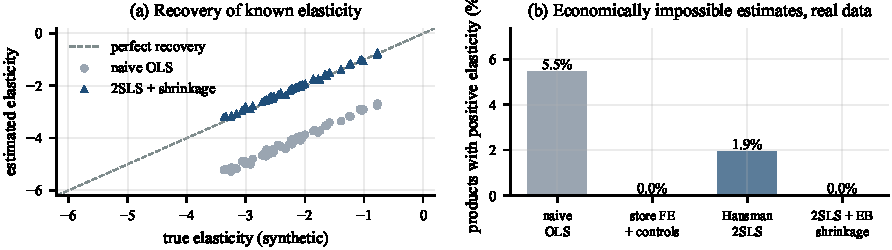
\includegraphics[width=\textwidth]{fig2_elasticity.pdf}
\caption{Elasticity. (a) Estimated against true value on the synthetic
replica. (b) Share of real-panel products with a positive, and therefore
impossible, elasticity.}
\label{fig:elast}
\end{figure*}

\begin{figure*}[!t]
\centering
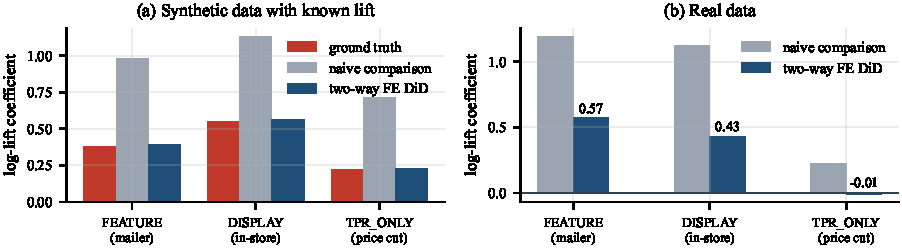
\includegraphics[width=\textwidth]{fig3_uplift.pdf}
\caption{Promotion uplift. (a) Difference-in-differences recovers the
planted lift; the naive comparison is inflated two- to three-fold. (b) The same
pattern on the real panel.}
\label{fig:uplift}
\end{figure*}

\subsection{Promotion uplift}
Fig.~\ref{fig:uplift}(a) compares estimates against planted truth: mean absolute
error across the three mechanics falls from $0.557$ to $0.010$, a factor of
$57$. Placebo coefficients of $0.001$, $-0.005$ and $0.000$ support the
parallel-trends assumption.

On the real panel the naive comparison again roughly doubles every estimate. The
corrected mailer lift is $0.572$ ($77.1\%$ in units) and the display lift
$0.432$ ($54.1\%$), each with standard error below $0.005$; placebo coefficients
are $-0.106$, $0.116$ and $-0.066$.

The temporary-price-reduction coefficient is $-0.007$, practically zero. This is
a consistency check rather than a null result: that mechanic is by definition a
price cut with no other support, so once price is controlled for nothing should
remain, and the model recovers that independently.

Combining causal lifts with estimated elasticities charges each promotion for
the margin it gives away. Under the stated cost assumption the display mechanic
is profitable for $60\%$ of products against a median break-even of $72\%$
volume lift; the price-cut mechanic is profitable for $2\%$, needing $99\%$ lift
while delivering $56\%$. Eight product--mechanic pairs priced below derived cost
are consistent with deliberate loss leaders, whose basket effects an item-level
model cannot see, and are flagged rather than called errors.

\subsection{Forecast accuracy}
Fig.~\ref{fig:fcst}(a) reports weighted absolute percentage error on the
held-out weeks: $0.294$ against $0.423$ for the strongest naive baseline, an
improvement of $30.5\%$. Reporting baselines matters, since an accuracy figure
quoted without them cannot be judged.

Residual bias after smearing is $+2.0\%$ against $-5.1\%$ uncorrected: the
correction slightly worsens WAPE while substantially reducing bias, the right
trade for a forecast feeding an inventory policy where under-prediction becomes
under-ordering. Fig.~\ref{fig:fcst}(b) shows accuracy tracking volume, from
$0.237$ for bag snacks at $18.6$ units per store-week to $0.405$ for oral
hygiene at $4.7$. On promoted store-weeks the forecast is $1.90\times$ the
counterfactual baseline, an independent cross-check on Section IV-B.

\begin{figure*}[!t]
\centering
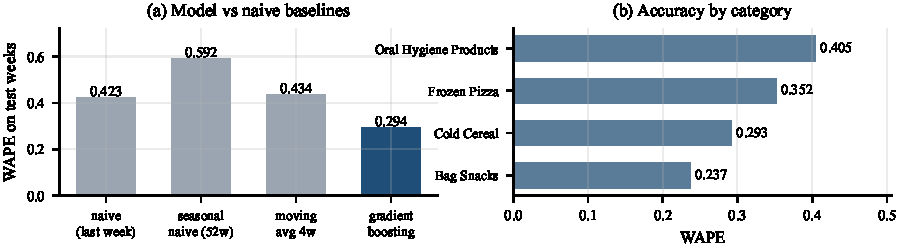
\includegraphics[width=\textwidth]{fig4_forecast.pdf}
\caption{Forecasting on held-out weeks 131--156. (a) Model against three
naive baselines. (b) Error by category.}
\label{fig:fcst}
\end{figure*}

\begin{figure*}[!t]
\centering
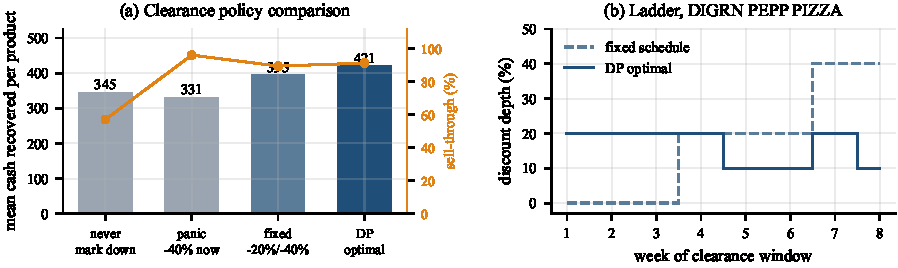
\includegraphics[width=\textwidth]{fig5_markdown.pdf}
\caption{Markdown. (a) Cash recovered and sell-through by policy.
(b) Optimal ladder against the fixed schedule; depth eases as stock depletes.}
\label{fig:md}
\end{figure*}

\subsection{Pricing and sensitivity}
The closed form agrees with a brute-force grid search to a maximum relative
difference of $3\times10^{-5}$. Of 54 products, 46 are elastic enough for an
interior optimum; for the other eight the guardrail sets the price. The
price-move cap binds for $85\%$ of products.

Applying the recommendations over the test weeks yields an expected gross-profit
increase of $11.7\%$, which must be reported with its caveat. Because unit cost
is derived from an assumed margin and the Lerner condition targets
$1/|\varepsilon|$, the recommendation partly reflects the gap between assumed
margin (mean $28.7\%$) and implied target (mean $45.6\%$). Re-solving across a
$\pm 5$ percentage-point band gives uplifts of $+175{,}477$, $+134{,}697$ and
$+99{,}787$ profit units, with $87$--$98\%$ of products still indicated for
increase. The direction is robust; the magnitude is not, so the honest result is
a range.

\subsection{Markdown and replenishment}
Fig.~\ref{fig:md} compares clearance policies over an eight-week horizon with
stock at fourteen weeks of baseline demand. The dynamic programme recovers
$6.6\%$ more cash than the fixed $-20\%/-40\%$ ladder and $21.9\%$ more than
never marking down, lifting sell-through from $57\%$ to $91\%$. Simulating the
computed policy reproduces its predicted value to within $0.12\%$, confirming
the recursion is solved correctly.

The optimal ladder in Fig.~\ref{fig:md}(b) \emph{reduces} depth in later weeks:
as stock depletes the urgency to clear falls, so price can be recovered. A fixed
schedule cannot express this because it never observes remaining inventory,
which is why it underperforms. The correlation between elasticity and weeks
discounted is $-0.68$: more elastic products earn their discounts back.

Table~\ref{tab:inv} reports replenishment cost over the held-out weeks across
1{,}324 store--product series. The forecast-driven policy cuts total cost by
$48.1\%$ against the textbook formula while reducing cover from $3.9$ to $2.8$
weeks and raising fill rate from $97.9\%$ to $99.1\%$. Less stock with better
service are usually opposing objectives; both improve because the forecast
indicates \emph{when} cover is needed rather than carrying it continuously.

The oracle row bounds what is attainable: perfect foresight would cut cost by
$98.3\%$, so the policy captures $49\%$ of the available saving. That ceiling is
more informative than the improvement alone. The saving concentrates where
demand is hardest to predict, rising from $7.6$ per series in the lowest
quartile of variability to $36.1$ in the highest.



\begin{table}[!t]
\caption{Replenishment cost on held-out weeks, 1{,}324 store--product series}
\label{tab:inv}
\centering
\footnotesize
\begin{tabular}{lrrrr}
\toprule
Policy & Holding & Stockout & Total & Fill \\
\midrule
Static normal (textbook)   & 19{,}740 & 23{,}682 & 43{,}422 & $97.9\%$ \\
Static empirical quantile  & 34{,}463 &  6{,}722 & 41{,}185 & $99.1\%$ \\
Forecast-driven (proposed) & 14{,}030 &  8{,}521 & 22{,}551 & $99.1\%$ \\
Oracle (perfect foresight) &      747 &        0 &      747 & $100\%$ \\
\bottomrule
\end{tabular}
\end{table}

\subsection{Limitations}
Unit cost, lead time, holding cost, salvage value and starting inventory appear
in no public retail panel and are stated assumptions; where a conclusion depends
materially on one it is reported across a range. Estimates rest on observed
rather than randomised variation, so causal claims are conditional on the
fixed-effects specification and are supported, not proved, by the placebo test.
The profit model is item-level and cannot see basket or traffic effects, which is
why below-cost promotions are flagged rather than judged. The replica validates
estimator mechanics under a known process; it cannot show that process describes
the real panel.

%=============================================================================
\section{Conclusion}

This work presents a retail decision system in which causal estimates of
elasticity and promotion uplift feed pricing, markdown and replenishment
modules, every decision being scored on held-out weeks against the heuristic it
would replace. Correcting for price endogeneity removes all impossible
elasticity estimates, and correcting for confounded promotion assignment reduces
log-lift error by a factor of $57$ against known ground truth. The decision
modules beat their incumbent baselines by $6.6\%$ in clearance cash recovery and
$48.1\%$ in inventory cost, the latter capturing just under half of what perfect
foresight could achieve.

The recurring finding is that the correction matters more than the model class:
in each module the largest gain came from removing a bias --- endogenous prices,
confounded promotions, retransformation under a log fit, sunk cost treated as
marginal --- rather than from a more elaborate learner. Ongoing work adds
per-recommendation attribution, closed-loop measurement of realised against
predicted profit, and an interface for adjusting the stated assumptions.

%=============================================================================
\begin{thebibliography}{00}

\bibitem{friedman2001} J. H. Friedman, ``Greedy function approximation: A
gradient boosting machine,'' \emph{Annals of Statistics}, vol. 29, no. 5,
pp. 1189--1232, 2001.

\bibitem{yang2025} Y. Yang, M. Wang, J. Wang \emph{et al.}, ``Multi-agent deep
reinforcement learning for integrated demand forecasting and inventory
optimization in sensor-enabled retail supply chains,'' \emph{Sensors}, vol. 25,
no. 8, p. 2428, 2025.

\bibitem{nevo2001} A. Nevo, ``Measuring market power in the ready-to-eat cereal
industry,'' \emph{Econometrica}, vol. 69, no. 2, pp. 307--342, 2001.

\bibitem{stock2005} J. H. Stock and M. Yogo, ``Testing for weak instruments in
linear IV regression,'' in \emph{Identification and Inference for Econometric
Models}, Cambridge Univ. Press, 2005, pp. 80--108.

\bibitem{efron1973} B. Efron and C. Morris, ``Stein's estimation rule and its
competitors---an empirical Bayes approach,'' \emph{J. Amer. Statist. Assoc.},
vol. 68, no. 341, pp. 117--130, 1973.

\bibitem{angrist2009} J. D. Angrist and J.-S. Pischke, \emph{Mostly Harmless
Econometrics: An Empiricist's Companion}. Princeton, NJ: Princeton Univ.
Press, 2009.

\bibitem{bertrand2004} M. Bertrand, E. Duflo, and S. Mullainathan, ``How much
should we trust differences-in-differences estimates?'' \emph{Quarterly Journal
of Economics}, vol. 119, no. 1, pp. 249--275, 2004.

\bibitem{lemmens2025} A. Lemmens, J. M. T. Roos, and S. Gabel,
``Personalization and targeting: How to experiment, learn and optimize,''
\emph{International Journal of Research in Marketing}, 2025.

\bibitem{lerner1934} A. P. Lerner, ``The concept of monopoly and the
measurement of monopoly power,'' \emph{Review of Economic Studies}, vol. 1,
no. 3, pp. 157--175, 1934.

\bibitem{gallego1994} G. Gallego and G. van Ryzin, ``Optimal dynamic pricing of
inventories with stochastic demand over finite horizons,'' \emph{Management
Science}, vol. 40, no. 8, pp. 999--1020, 1994.

\bibitem{gijsbrechts2022} J. Gijsbrechts, R. N. Boute, J. A. Van Mieghem, and
D. J. Zhang, ``Can deep reinforcement learning improve inventory management?
Performance on lost sales, dual-sourcing, and multi-echelon problems,''
\emph{Manufacturing \& Service Operations Management}, vol. 24, no. 3,
pp. 1349--1368, 2022.

\bibitem{assad2024} S. Assad, R. Clark, D. Ershov, and L. Xu, ``Algorithmic
pricing and competition: Empirical evidence from the German retail gasoline
market,'' \emph{Journal of Political Economy}, vol. 132, no. 3,
pp. 723--771, 2024.

\bibitem{fish2024} S. Fish, Y. A. Gonczarowski, and R. I. Shorrer,
``Algorithmic collusion by large language models,'' arXiv:2404.00806, 2024.

\bibitem{debock2024} K. W. De Bock, K. Coussement, A. De Caigny \emph{et al.},
``Explainable AI for operational research: A defining framework, methods,
applications, and a research agenda,'' \emph{European Journal of Operational
Research}, vol. 314, no. 2, pp. 415--439, 2024.

\bibitem{duan1983} N. Duan, ``Smearing estimate: A nonparametric
retransformation method,'' \emph{J. Amer. Statist. Assoc.}, vol. 78, no. 383,
pp. 605--610, 1983.

\bibitem{dunnhumby} dunnhumby, ``Breakfast at the Frat: A time series
analysis,'' dunnhumby Source Files. [Online]. Available:
\url{https://www.dunnhumby.com/source-files/}

\end{thebibliography}

\balance

%=============================================================================
% APPENDIX - beyond the six-page main paper
%=============================================================================
\ifincludecode

\onecolumn
\appendices
\section*{APPENDIX --- SIMULATION CODE}

The complete implementation is listed below, with modules in execution order.
Each listing is read directly from the source file used to produce the results
in this paper, so the code shown is the code that was run.

\subsection*{A. Configuration and schema contract}
\codefile{src/config.py}{config.py}
\codefile{src/schema.py}{schema.py}

\subsection*{B. Synthetic replica generator}
\codefile{src/make\_synthetic\_frat.py}{make_synthetic_frat.py}

\subsection*{C. Data loading and preprocessing}
\codefile{src/data\_loader.py}{data_loader.py}

\subsection*{D. Price elasticity estimation}
\codefile{src/elasticity.py}{elasticity.py}

\subsection*{E. Causal promotion uplift}
\codefile{src/uplift.py}{uplift.py}

\subsection*{F. Demand forecasting}
\codefile{src/forecast.py}{forecast.py}

\subsection*{G. Constrained price optimisation}
\codefile{src/pricing.py}{pricing.py}

\subsection*{H. Markdown optimisation}
\codefile{src/markdown.py}{markdown.py}

\subsection*{I. Inventory replenishment}
\codefile{src/inventory.py}{inventory.py}

\subsection*{J. Figure generation}
\codefile{src/make\_figures.py}{make_figures.py}

\fi

\end{document}
